
%(BEGIN_QUESTION)
% Copyright 2011, Tony R. Kuphaldt, released under the Creative Commons Attribution License (v 1.0)
% This means you may do almost anything with this work of mine, so long as you give me proper credit

Examine this valve positioner illustration, and then answer the following questions about it:

$$\includegraphics[width=15.5cm]{i01073x01.eps}$$

\vskip 20pt

If a technician lengthened the link connecting the positioner's beam to the valve stem bracket, what effect would this have on the calibration of the whole control valve assembly?  Would it introduce a {\it zero} shift, a {\it span} shift, or a change in {\it linearity}?  Be as detailed as you can in your answer.

\vskip 30pt

If a technician replaced the main spring in the valve actuator with one that was stiffer (i.e. a larger $k$ spring constant), what effect would this have on the calibration of the whole control valve assembly?  Would it introduce a {\it zero} shift, a {\it span} shift, or a change in {\it linearity}?  Be as detailed as you can in your answer.

\vskip 30pt

Suppose this very same positioner mechanism were attached to a direct-acting actuator (air to move the stem down) rather than a reverse-acting actuator (air to move the stem up) as shown here.  What, if anything, would have to be altered in the positioner mechanism to make it function properly with this different actuator?  Explain the rationale for any mechanism changes that would have to be made.

\vfil 

\underbar{file i01073}
\eject
%(END_QUESTION)





%(BEGIN_ANSWER)

This is a graded question -- no answers or hints given!

%(END_ANSWER)





%(BEGIN_NOTES)

The {\it very first step} in analyzing any pneumatic mechanism should be to determine its nature as being either {\it force-balance} or {\it motion-balance}.  To do this, apply the simplifying assumption that negative feedback will always hold the nozzle/baffle gap will constant, and then see if the various components within the device are able to move at all.  If motion is possible, then the mechanism is {\it motion-balance} and must be analyzed from the perspective of how far the parts will move.  If no motion is possible, then the mechanism is {\it force-balance} and must be analyzed from the perspective of how hard the parts will push on each other.

This particular valve positioner mechanism is clearly {\it motion-balance}, as the input (control signal) bellows and valve stem must both move in see-saw fashion to maintain a constant beam/nozzle gap.  Therefore, we must analyze this mechanism in terms of motion (i.e. how far must the parts move).

\vskip 10pt

Lengthening the connecting link between the valve stem and the beam adds distance between those two components, which is equivalent to {\it adding motion} to the mechanism.  The positioner mechanism now ``thinks'' the valve is farther closed than it actually is.  If this is difficult for you to envision, just imagine the valve being at its fully-closed position and then lengthening the link.  Doing so would attempt to push the beam toward the nozzle, increasing pressure in the mechanism and applying more air pressure to the actuator to move the valve open.  Since we know that a {\it zero} shift is always additive or subtractive to an instrument's calibration, and we see here that a longer link definitely {\it adds} motion to the system, we may conclude that this change will shift the zero of the valve positioner.

\vskip 10pt

A stiffer spring would have {\it no effect} on the calibration of the assembly, assuming the supply pressure to the positioner was still adequate to fully lift the stem.  Remember that {\it the job of a valve positioner is to apply as much or as little air pressure is necessary to get the valve to move to the desired stem position}.  Increasing the valve spring's stiffness merely increases the amount of air pressure necessary to open the valve to any given stem position.  So long as the positioner has the ability to deliver the necessary air pressure, the valve will still move the way it should.

\vskip 10pt

For a direct-acting actuator, the nozzle would have to be moved to the other side of the beam, so that a rising stem would result in more pressure sent to the actuator rather than less.  The negative-feedback relationship of the nozzle/beam gap to the effect of applied air to the actuator must be maintained, or else the positioner will fail to function at all.

%INDEX% Final Control Elements, valve: positioner

%(END_NOTES)


